\begin{figure}[H]
  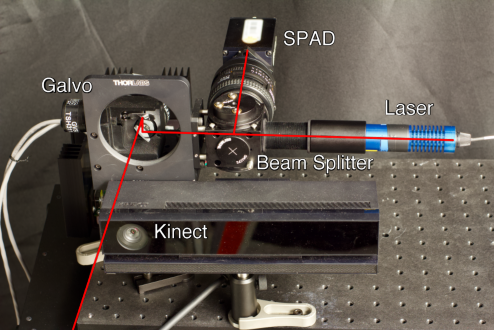
\includegraphics[width=\linewidth]{prototype_single_col.png}
  \caption{Prototype scanning setup. The pulsed light from the laser travels
    through a beam splitter before being guided by the galvo to the scene.
    Returning light is measured by the single-pixel SPAD. The RGB camera of a
    Kinect v2 is used to capture the monocular RGB image (the depth camera is
    not used)}
  \label{fig:prototype}
\end{figure}

%%%%%%%%%%%%%%%%%%%%%%%%%%%%%%%%%%%%%%%%%%%%%%%%%%%%%%%%%%%%%%%%
\subsection{Prototype RGB-SPAD Camera Hardware}

% The laser operates at 450~nm with a pulse repetition rate of 25~MHz with a peak power of 450~mW and average power of 0.5~mW.

As shown in Figure~\ref{fig:prototype}, our prototype camera comprises a color camera (Microsoft Kinect v2), a single-pixel SPAD (\textcolor{red}{DETAILS}), a laser (ALPHALAS PICOPOWER-LD-450-50), and a two-axis galvanometer mirror system (Thorlabs GVS012). The laser operates at 670~nm with a pulse repetition rate of 20~MHz with a peak power of 450~mW and average power of 0.5~mW. The SPAD records temporal histograms with 65536 bins, each corresponding to a time window of 4~ps. SPAD and laser are co-axially aligned using a beam splitter (Thorlabs PBS251). The full width at half maximum (FWHM) of the combined laser pulse width and SPAD jitter is about 70~ps, allowing the system to record depth map with an accuracy of about 1~cm. A National Instruments data acquisition device (NI-DAQ USB-6343) provides synchronization signals for the galvos, SPAD, and laser. The ground truth depth map is raster-scanned at a resolution of $512 \times 512$ pixels. The single-pixel, diffused SPAD measurement is generated by summing all of these measurements for a specific scene. This allows us to validate the accuracy of the proposed histogram matching algorithm that only uses the single histogram of the diffused SPAD and compare it with ground truth. Monocular depth estimation is calculated using the RGB image captured by the Kinect v2.

\textcolor{red}{Mark, please write a short paragraph on calibration details, including any warping of the SPAD histograms you did to compensate for the offset in camera and SPAD position.}

Missing:
%
\begin{itemize}
\item resolution of ground truth depth
\item RGB resolution
\item do we also have Kinect depth maps for comparison? (yes) kinect resolution: RGB is 1920x1080 and depth camera is 512x424
\end{itemize}

%%%%%%%%%%%%%%%%%%%%%%%%%%%%%%%%%%%%%%%%%%%%%%%%%%%%%%%%%%%%%%%%
\subsection{Experimental Results}
